\documentclass[../main]{subfiles}

\questiontrue
\solutiontrue

\begin{document}
    \ifquestion
    
    \section{Let There Be Light!}
	
	
The Kamoto Universe is a universe where the laws of physics are nearly identical to ours, with one exception: gravitational attraction follows the relation:

\[\vec{F}_{ij}=-Gm_im_j(\vec{r}_{j}-\vec{r}_{i})\]

where \(\vec{F}_{ij}\) is the force exerted on \(j\) by \(i\). This purely classical universe (which lacks quantum mechanics, relativity, etc.) has a total mass \(M\) and an intrinsic gravitational constant \(G\).

\parte{A}{Age of the Universe}

\ut{A.1}{Resultant Force in the Center of Mass Reference Frame}

Write the resultant force in the center of mass frame due to the gravitational action of all particles in this universe on a particle \(j\).

\ut{A.2}{Equation of Motion}

Derive the equation of motion for this particle.

\ut{A.3}{Estimating the Universe's Lifetime}

Estimate the lifetime of this universe considering it has the same parameters as our universe (\(M=10^{54}kg\) and \(G=6.67 \cdot 10^{-11} N/(kg^2\cdot m)\)).

\parte{B}{Kepler's Laws}

In the following items, some orbital properties of this atypical universe will be analyzed.

\ut{B.1}{Center of Mass and Center of Gravity}

In our universe, the center of gravity of a body does not necessarily coincide with its center of mass (for most shapes, it does not). Discuss the relationship between the center of mass and the center of gravity in the Kamoto universe.

Consider a particle of mass \(m\) orbiting \(M\) (with \(m \ll M\)):

\ut{B.2}{Second Law of Kepler}

Prove that Kepler’s second law remains valid in this scenario and find an expression for the areal velocity (area swept by the position vector per unit time) as a function of the angular momentum of the particle \(m\), denoted as \(L\).

\ut{B.3}{Orbital Shape}

Determine the shape of \(m\)'s orbit (analogous to Kepler’s first law).

\ut{B.4}{Third Law of Kepler Equivalent}

Find the analog to Kepler’s third law for this universe, proving that:
\[T=a^n k(M)\]
where \(a\) is some measure of the orbital shape, \(T\) is the period, and \(k(M)\) is a constant depending only on the central mass \(M\).

For example, in our universe, \(n=\frac{3}{2}\) and \(k(M)=\sqrt{\frac{4\pi^2}{GM}}\). Determine \(n\) and \(k(M)\) for the Kamoto universe.

\parte{C}{Orbital Transfers}

In the following items, an orbital transfer situation will be analyzed.

\ut{C.1}{Orbital Velocity at Extremes}

A team of astronauts is orbiting a central mass \(M\) in an elliptical orbit with semi-major axis \(a\) and semi-minor axis \(b\). Derive an equation for the orbital velocity when the spacecraft is at its maximum distance from the planet (\(v_a\)) and at its minimum distance (\(v_b\)).

\ut{C.2}{Multi-Step Orbital Transfer}

The team aims to reach a second circular orbit of radius \(\alpha R\) (with \(\alpha>1\)). The method used involves \(n\) elliptical transfers such that the semi-major axis of ellipse \(i\) corresponds to the semi-minor axis of ellipse \(i+1\), as shown in Figure \ref{fig:trielipse}.

	\begin{figure}[htpb]
	    \centering
	   
\tikzset{every picture/.style={line width=0.75pt}} %set default line width to 0.75pt        

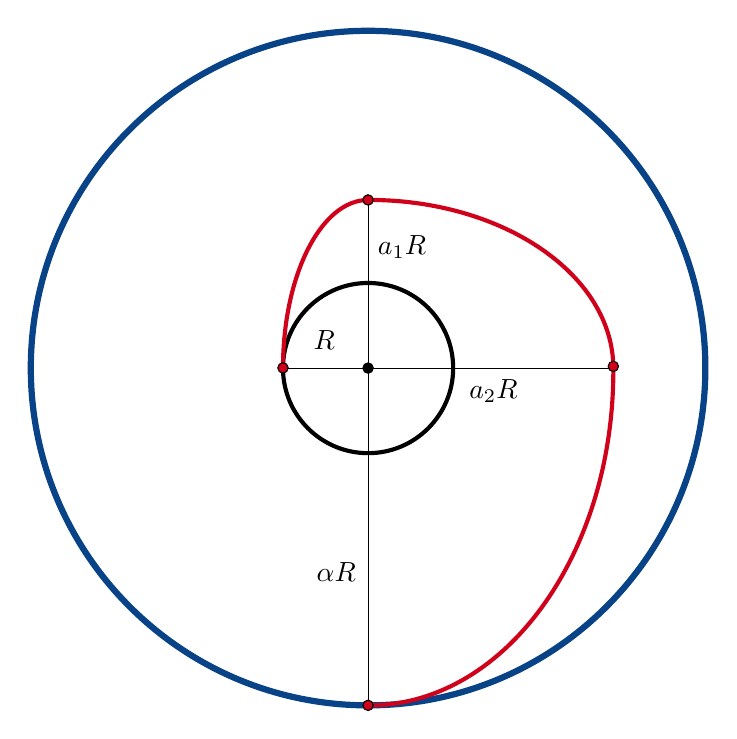
\begin{tikzpicture}[x=0.75pt,y=0.75pt,yscale=-1,xscale=1]
%uncomment if require: \path (0,408); %set diagram left start at 0, and has height of 408

%Shape: Circle [id:dp04985988715130163] 
\draw  [color={rgb, 255:red, 8; green, 66; blue, 135 }  ,draw opacity=1 ][line width=2.25]  (191,204.17) .. controls (191,114.43) and (263.75,41.67) .. (353.5,41.67) .. controls (443.25,41.67) and (516,114.43) .. (516,204.17) .. controls (516,293.92) and (443.25,366.67) .. (353.5,366.67) .. controls (263.75,366.67) and (191,293.92) .. (191,204.17) -- cycle ;
%Shape: Circle [id:dp7782171078596141] 
\draw  [line width=1.5]  (312.5,204.17) .. controls (312.5,181.53) and (330.86,163.17) .. (353.5,163.17) .. controls (376.14,163.17) and (394.5,181.53) .. (394.5,204.17) .. controls (394.5,226.82) and (376.14,245.17) .. (353.5,245.17) .. controls (330.86,245.17) and (312.5,226.82) .. (312.5,204.17) -- cycle ;
%Straight Lines [id:da6463203796073529] 
\draw    (312.5,204.17) -- (353.5,204.17) ;
%Straight Lines [id:da3087370137326533] 
\draw    (353.5,123.17) -- (353.5,204.17) ;
%Straight Lines [id:da02530793507398177] 
\draw    (353.5,204.17) -- (472,204.17) ;
%Straight Lines [id:da4217033584107446] 
\draw    (353.5,204.17) -- (353.5,366.67) ;
%Shape: Circle [id:dp17963483851145057] 
\draw  [fill={rgb, 255:red, 0; green, 0; blue, 0 }  ,fill opacity=1 ] (353.44,201.67) .. controls (354.82,201.64) and (355.97,202.73) .. (356,204.11) .. controls (356.03,205.49) and (354.94,206.64) .. (353.56,206.67) .. controls (352.18,206.7) and (351.03,205.61) .. (351,204.23) .. controls (350.97,202.85) and (352.06,201.7) .. (353.44,201.67) -- cycle ;
%Shape: Arc [id:dp022695648206921604] 
\draw  [draw opacity=0][line width=1.5]  (312.5,204.1) .. controls (312.55,159.38) and (330.89,123.17) .. (353.5,123.17) -- (353.5,204.3) -- cycle ; \draw  [color={rgb, 255:red, 208; green, 2; blue, 27 }  ,draw opacity=1 ][line width=1.5]  (312.5,204.1) .. controls (312.55,159.38) and (330.89,123.17) .. (353.5,123.17) ;  
%Shape: Arc [id:dp25786173838203585] 
\draw  [draw opacity=0][line width=1.5]  (352.65,123.18) .. controls (353.1,123.17) and (353.55,123.17) .. (354,123.17) .. controls (418.99,123.17) and (471.67,159.51) .. (471.67,204.34) -- (354,204.34) -- cycle ; \draw  [color={rgb, 255:red, 208; green, 2; blue, 27 }  ,draw opacity=1 ][line width=1.5]  (352.65,123.18) .. controls (353.1,123.17) and (353.55,123.17) .. (354,123.17) .. controls (418.99,123.17) and (471.67,159.51) .. (471.67,204.34) ;  
%Shape: Arc [id:dp8008993144301884] 
\draw  [draw opacity=0][line width=1.5]  (471.66,203.35) .. controls (471.66,204) and (471.67,204.65) .. (471.67,205.3) .. controls (471.67,294.42) and (419.02,366.67) .. (354.08,366.67) .. controls (353.68,366.67) and (353.28,366.67) .. (352.87,366.66) -- (354.08,205.3) -- cycle ; \draw  [color={rgb, 255:red, 208; green, 2; blue, 27 }  ,draw opacity=1 ][line width=1.5]  (471.66,203.35) .. controls (471.66,204) and (471.67,204.65) .. (471.67,205.3) .. controls (471.67,294.42) and (419.02,366.67) .. (354.08,366.67) .. controls (353.68,366.67) and (353.28,366.67) .. (352.87,366.66) ;  
%Shape: Circle [id:dp5538965088814416] 
\draw  [color={rgb, 255:red, 0; green, 0; blue, 0 }  ,draw opacity=1 ][fill={rgb, 255:red, 208; green, 2; blue, 27 }  ,fill opacity=1 ] (312.44,201.6) .. controls (313.82,201.57) and (314.97,202.66) .. (315,204.04) .. controls (315.03,205.42) and (313.94,206.56) .. (312.56,206.6) .. controls (311.18,206.63) and (310.03,205.53) .. (310,204.15) .. controls (309.97,202.77) and (311.06,201.63) .. (312.44,201.6) -- cycle ;
%Shape: Circle [id:dp7551305949674694] 
\draw  [color={rgb, 255:red, 0; green, 0; blue, 0 }  ,draw opacity=1 ][fill={rgb, 255:red, 208; green, 2; blue, 27 }  ,fill opacity=1 ] (471.6,200.85) .. controls (472.98,200.82) and (474.13,201.91) .. (474.16,203.29) .. controls (474.19,204.67) and (473.1,205.81) .. (471.72,205.85) .. controls (470.34,205.88) and (469.19,204.79) .. (469.16,203.41) .. controls (469.13,202.02) and (470.22,200.88) .. (471.6,200.85) -- cycle ;
%Shape: Circle [id:dp27272397998397424] 
\draw  [color={rgb, 255:red, 0; green, 0; blue, 0 }  ,draw opacity=1 ][fill={rgb, 255:red, 208; green, 2; blue, 27 }  ,fill opacity=1 ] (353.44,120.67) .. controls (354.82,120.64) and (355.97,121.73) .. (356,123.11) .. controls (356.03,124.49) and (354.94,125.64) .. (353.56,125.67) .. controls (352.18,125.7) and (351.03,124.61) .. (351,123.23) .. controls (350.97,121.85) and (352.06,120.7) .. (353.44,120.67) -- cycle ;
%Shape: Circle [id:dp8805004193971959] 
\draw  [color={rgb, 255:red, 0; green, 0; blue, 0 }  ,draw opacity=1 ][fill={rgb, 255:red, 208; green, 2; blue, 27 }  ,fill opacity=1 ] (353.44,364.17) .. controls (354.82,364.14) and (355.97,365.23) .. (356,366.61) .. controls (356.03,367.99) and (354.94,369.14) .. (353.56,369.17) .. controls (352.18,369.2) and (351.03,368.11) .. (351,366.73) .. controls (350.97,365.35) and (352.06,364.2) .. (353.44,364.17) -- cycle ;

% Text Node
\draw (326,185.07) node [anchor=north west][inner sep=0.75pt]    {$R$};
% Text Node
\draw (357,139.07) node [anchor=north west][inner sep=0.75pt]    {$a_{1} R$};
% Text Node
\draw (401,208.57) node [anchor=north west][inner sep=0.75pt]    {$a_{2} R$};
% Text Node
\draw (327.5,296.57) node [anchor=north west][inner sep=0.75pt]    {$\alpha R$};


\end{tikzpicture}
	    \caption{Scheme showing a transfer with $n=3$}
	    \label{fig:trielipse}
	\end{figure}

	Determine the total $\Delta v_T$, that is, the sum of all $\Delta v_i$ needed to complete the transfer.
	
	\ut{C.3} Determine the time taken for complete orbital transfer.
	
	
	\clearpage
    
    
    \fi
    
    \ifsolution
    
    \section{Let There Be Light!}

\parte{A}{Age of the Universe}

\ut{A.1} To find the resultant force on particle $j$, we simply sum vectorially all the forces acting on it:  
\[
\vec{F}_{res}=\sum_{i \ne j}(-Gm_im_j(\vec{r}_{j}-\vec{r}_{i}))
\]  

Note: We sum over all possible indices $i$, except for $j$, because the particle does not exert a force on itself.  

Recalling that $m_j$ and $r_j$ are constants (the mass and position of a chosen particle) and expanding, we obtain:  

\[
\vec{F}_{res}=-Gm_j\sum_{i \ne j}(m_i(\vec{r}_{j}-\vec{r}_{i}))
\]  

\[
\vec{F}_{res}=-Gm_j\left(\sum_{i \ne j}(m_i\vec{r}_{j})-\sum_{i \ne j}(m_i\vec{r}_{i})\right)
\]  

\[
\vec{F}_{res}=-Gm_j\left(\vec{r}_{j}\sum_{i \ne j}(m_i)-\sum_{i \ne j}(m_i\vec{r}_{i})\right)
\]  

Now note that $\sum_{i \ne j}(m_i)$ is the sum of the masses of all the particles in the universe except for $j$, so $\sum_{i \ne j}(m_i)=M-m_j$. Thus:  

\[
\vec{F}_{res}=-Gm_j\left(\vec{r}_{j}(M-m_j)-\sum_{i \ne j}(m_i\vec{r}_{i})\right)
\]  

\[
\vec{F}_{res}=-Gm_j\left(M\vec{r}_{j}-m_j\vec{r}_{j}-\sum_{i \ne j}(m_i\vec{r}_{i})\right)
\]  

Grouping $m_j\vec{r}_{j}$ into the summation, we get:  

\[
\vec{F}_{res}=-Gm_j\left(M\vec{r}_{j}-\sum_{i}(m_i\vec{r}_{i})\right)
\]  

Since these positions refer to the center of mass, we know from the definition of the center of mass that $\sum_{i}(m_i\vec{r}_{i})=0$, so:  

\[
\vec{F}_{res}=-GMm_j\vec{r}_{j}
\]  

\ut{A.2} Applying Newton’s second law to $m_j$: $\vec{F}_{res}=m_j\vec{a}_{res}$, where $\vec{a}_{res}$ is the total acceleration of $j$ in the center of mass reference frame. Finally:  

\[
\vec{a}_{res}=-GM\vec{r}_{j}
\]  

\ut{A.3} Note that the acceleration varies linearly with the position of the particle, so we have a force of the type $F=-kx$, meaning the particle undergoes simple harmonic motion (SHM). Also, observe that the result found in item (b) does not depend on mass, so ALL particles will follow this SHM (since they all start from the same point at the beginning of the universe).  

Thus, we need to find half of the period of SHM (only half because the particles start at position 0, reach the maximum, and return to 0).  

\[
a_{res}=-\omega^2 r_j
\]  

\[
T=\frac{1}{2}\left(\frac{2\pi}{\omega}\right)
\]  

\[
\omega=\sqrt{GM}
\]  

\[
\therefore T=\sqrt{\frac{\pi^2}{GM}} \approx 3.85 \cdot 10^{-22}s
\]  

\parte{B}{Kepler's Laws}

\ut{B.1} As demonstrated in item \textbf{A.2)}, the total acceleration generated by a rigid body on a test mass is given by:  

\[
\vec{a}=GM\vec{r}
\]  

Where $\vec{r}$ is the position vector originating from the center of mass of the rigid body. From this relation, we see that the center of application of gravitational force coincides with the center of mass of the body! Thus, unlike in our universe, we can consider the effect of a body of any shape or size as that of a point mass located at the system's center of mass.  

\ut{B.2} Consider a moment when the body $m$ is at a distance $r$ from $M$ and the angle between the velocity $v$ of $m$ and $r$ is $\theta$. After an infinitesimal interval $dt$, the body will travel a distance $vdt$ in the direction and sense of the velocity vector. Thus, the radial vector will have swept an area in the shape of a triangle, and we can calculate this area:  

\[
dA=\frac{1}{2}rvdt\sin{\theta} \rightarrow \frac{dA}{dt}=v_{A}=\frac{1}{2m}mvr\sin{\theta}=\frac{L}{2m}
\]  

Since $L$ is a conserved quantity (because the gravitational force is a central force, meaning it points in the same direction as the position vector relative to $M$), we know that $v_A$ is constant and equal to $\dfrac{L}{2m}$.  

\ut{B.3} Write the acceleration and position vectors of the body:  

\[
\begin{bmatrix}
a_x \\
a_y \\
\end{bmatrix}
= -GM
\begin{bmatrix}
x\\
y\\
\end{bmatrix}
\]  

From this, we see that, by associating each component:  

\[
\begin{cases}
a_x=-GMx\\
a_y=-GMy\\
\end{cases}
\]  

This implies that the body undergoes SHM with the same period in each axis:  

\[
\begin{cases}
x=A\cos{(\sqrt{GM}t+\phi_x)}\\
y=B\cos{(\sqrt{GM}t+\phi_y)}\\
\end{cases}
\]  

For simplification, let \(\sqrt{GM}=\omega\). Now we will use an algebraic trick to find the equation of the curve:  

\[
\cos{(\omega t+\phi_x-\omega t+\phi_y)}=\cos{(\omega t+\phi_x)}\cos{(\omega t+\phi_y)}+\sin{(\omega t+\phi_x)}\sin{(\omega t+\phi_y)}
\]

\[
\therefore \cos{(\omega t+\phi_x-\omega t+\phi_y)}=\cos{(\phi_x-\phi_y)}=\frac{x}{A}\frac{y}{B}+\sqrt{1-\frac{x^2}{A^2}}\sqrt{1-\frac{y^2}{B^2}}
\]

Let \(\cos{(\phi_x-\phi_y)}=k\):

\[
\sqrt{1-\frac{x^2}{A^2}-\frac{y^2}{B^2}+\frac{x^2y^2}{A^2B^2}}=k-\frac{x}{A}\frac{y}{B}
\]

Simplifying, we find:

\[
\frac{x^2}{A^2}+\frac{y^2}{B^2}-\frac{2kxy}{AB}+k^2-1=0
\]

The previous equation is nothing more than the equation of a rotated conic! Since the motion of \(m\) is periodic, it cannot be parabolic or hyperbolic, so we infer that it must be an ellipse!

\ut{B.4} 
Note that the period can be found in the same way as did previously, that is:

\[
T=2\pi\sqrt{\frac{1}{GM}}
\]

Thus:

\[
n=0 \text{ and } k(M)=\sqrt{\frac{4\pi^2}{GM}}
\]

\parte{C}{Orbital Transfers}

\ut{C.1}

First, define the coordinate axes: \(y\) represents the Cartesian axis containing the minor axis of the ellipse, and \(x\) represents the Cartesian axis containing the major axis of the ellipse. Notice the following: the velocity of the body in a Cartesian axis is maximal when it is at the maximum amplitude in the complementary elliptical axis. For example, the velocity when the body passes through the major axis equals the maximum velocity of the simple harmonic motion (SHM) in the \(y\) axis, as illustrated in the following scheme:
	
	\begin{figure}[htpb]
	    \centering
	    

\tikzset{every picture/.style={line width=0.75pt}} %set default line width to 0.75pt        

\begin{tikzpicture}[x=0.75pt,y=0.75pt,yscale=-1,xscale=1]
%uncomment if require: \path (0,408); %set diagram left start at 0, and has height of 408

%Shape: Ellipse [id:dp8640552728904485] 
\draw  [color={rgb, 255:red, 208; green, 2; blue, 27 }  ,draw opacity=1 ] (129.33,198.84) .. controls (129.33,140.03) and (211.64,92.34) .. (313.17,92.34) .. controls (414.7,92.34) and (497,140.03) .. (497,198.84) .. controls (497,257.66) and (414.7,305.34) .. (313.17,305.34) .. controls (211.64,305.34) and (129.33,257.66) .. (129.33,198.84) -- cycle ;
%Shape: Circle [id:dp349521589849652] 
\draw  [fill={rgb, 255:red, 0; green, 0; blue, 0 }  ,fill opacity=1 ] (313.11,89.84) .. controls (314.49,89.81) and (315.63,90.91) .. (315.67,92.29) .. controls (315.7,93.67) and (314.61,94.81) .. (313.22,94.84) .. controls (311.84,94.88) and (310.7,93.78) .. (310.67,92.4) .. controls (310.64,91.02) and (311.73,89.88) .. (313.11,89.84) -- cycle ;
%Shape: Circle [id:dp8356813579235054] 
\draw  [fill={rgb, 255:red, 0; green, 0; blue, 0 }  ,fill opacity=1 ] (496.94,196.34) .. controls (498.32,196.31) and (499.47,197.41) .. (499.5,198.79) .. controls (499.53,200.17) and (498.44,201.31) .. (497.06,201.34) .. controls (495.68,201.38) and (494.53,200.28) .. (494.5,198.9) .. controls (494.47,197.52) and (495.56,196.38) .. (496.94,196.34) -- cycle ;
%Straight Lines [id:da9469502895388491] 
\draw  [dash pattern={on 0.84pt off 2.51pt}]  (129.33,52.68) -- (129.33,198.84) ;
%Straight Lines [id:da5161043163028576] 
\draw  [dash pattern={on 0.84pt off 2.51pt}]  (497,52.68) -- (497,198.84) ;
%Straight Lines [id:da3523934744666015] 
\draw    (131.33,52.68) -- (495,52.68) ;
\draw [shift={(497,52.68)}, rotate = 180] [color={rgb, 255:red, 0; green, 0; blue, 0 }  ][line width=0.75]    (10.93,-3.29) .. controls (6.95,-1.4) and (3.31,-0.3) .. (0,0) .. controls (3.31,0.3) and (6.95,1.4) .. (10.93,3.29)   ;
\draw [shift={(129.33,52.68)}, rotate = 0] [color={rgb, 255:red, 0; green, 0; blue, 0 }  ][line width=0.75]    (10.93,-3.29) .. controls (6.95,-1.4) and (3.31,-0.3) .. (0,0) .. controls (3.31,0.3) and (6.95,1.4) .. (10.93,3.29)   ;
%Straight Lines [id:da6100311961733937] 
\draw  [dash pattern={on 0.84pt off 2.51pt}]  (313.17,92.34) -- (66.33,92.34) ;
%Straight Lines [id:da9157002695032459] 
\draw    (66.33,303.34) -- (66.33,94.34) ;
\draw [shift={(66.33,92.34)}, rotate = 90] [color={rgb, 255:red, 0; green, 0; blue, 0 }  ][line width=0.75]    (10.93,-3.29) .. controls (6.95,-1.4) and (3.31,-0.3) .. (0,0) .. controls (3.31,0.3) and (6.95,1.4) .. (10.93,3.29)   ;
\draw [shift={(66.33,305.34)}, rotate = 270] [color={rgb, 255:red, 0; green, 0; blue, 0 }  ][line width=0.75]    (10.93,-3.29) .. controls (6.95,-1.4) and (3.31,-0.3) .. (0,0) .. controls (3.31,0.3) and (6.95,1.4) .. (10.93,3.29)   ;
%Straight Lines [id:da9415833374734444] 
\draw    (313.17,92.34) -- (437,92.34) ;
\draw [shift={(439,92.34)}, rotate = 180] [color={rgb, 255:red, 0; green, 0; blue, 0 }  ][line width=0.75]    (10.93,-3.29) .. controls (6.95,-1.4) and (3.31,-0.3) .. (0,0) .. controls (3.31,0.3) and (6.95,1.4) .. (10.93,3.29)   ;
%Straight Lines [id:da22479759819812628] 
\draw  [dash pattern={on 0.84pt off 2.51pt}]  (313.17,305.34) -- (66.33,305.34) ;
%Straight Lines [id:da07188196125980229] 
\draw    (497,198.84) -- (497,266.68) ;
\draw [shift={(497,268.68)}, rotate = 270] [color={rgb, 255:red, 0; green, 0; blue, 0 }  ][line width=0.75]    (10.93,-3.29) .. controls (6.95,-1.4) and (3.31,-0.3) .. (0,0) .. controls (3.31,0.3) and (6.95,1.4) .. (10.93,3.29)   ;
%Shape: Circle [id:dp04566684303860358] 
\draw  [color={rgb, 255:red, 0; green, 0; blue, 0 }  ,draw opacity=1 ][fill={rgb, 255:red, 208; green, 2; blue, 27 }  ,fill opacity=1 ] (313.11,196.34) .. controls (314.49,196.31) and (315.63,197.41) .. (315.67,198.79) .. controls (315.7,200.17) and (314.61,201.31) .. (313.22,201.34) .. controls (311.84,201.38) and (310.7,200.28) .. (310.67,198.9) .. controls (310.64,197.52) and (311.73,196.38) .. (313.11,196.34) -- cycle ;

% Text Node
\draw (302.67,32.4) node [anchor=north west][inner sep=0.75pt]    {$2a$};
% Text Node
\draw (44.67,177.74) node [anchor=north west][inner sep=0.75pt]    {$2b$};
% Text Node
\draw (500,215.41) node [anchor=north west][inner sep=0.75pt]  [font=\Large]  {$v_{a}$};
% Text Node
\draw (361.33,62.74) node [anchor=north west][inner sep=0.75pt]  [font=\Large]  {$v_{b}$};


\end{tikzpicture}
        \caption{Representation of the orbit and apoastron and periastron velocities}
	    \label{fig:elipsi}
	\end{figure}
	

    From the equations obtained in item \textbf{B.2)}, we know that the velocity equation in the \(y\) axis can be written as: \(v_y=-B\sqrt{GM}\sin{(\sqrt{GM}t+\phi_b)}\). In the case where the spacecraft is at the semi-major axis, the velocity in the \(y\) axis is maximal, so \(v_a=B\sqrt{GM}\). Notice that the value of \(B\) is nothing more than the amplitude of the simple harmonic motion (SHM) in the \(y\) axis, so we see that \(B=b\), thus:  

\[
v_a=b\sqrt{GM}
\]

Similarly:  

\[
v_b=a\sqrt{GM}
\]

\ut{C.2} By convention, we will call \(R\sqrt{GM}\) as \(v\) in this solution. Consider the diagram proposed by the statement (Figure \ref{fig:trielipse}):

	\begin{figure}[htpb]
	    \centering
	   
\tikzset{every picture/.style={line width=0.75pt}} %set default line width to 0.75pt        

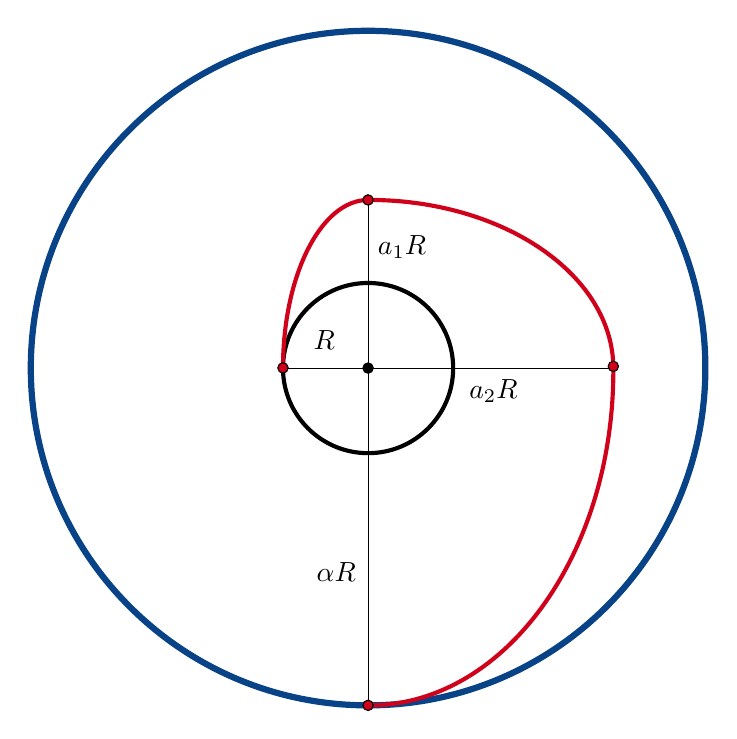
\begin{tikzpicture}[x=0.75pt,y=0.75pt,yscale=-1,xscale=1]
%uncomment if require: \path (0,408); %set diagram left start at 0, and has height of 408

%Shape: Circle [id:dp04985988715130163] 
\draw  [color={rgb, 255:red, 8; green, 66; blue, 135 }  ,draw opacity=1 ][line width=2.25]  (191,204.17) .. controls (191,114.43) and (263.75,41.67) .. (353.5,41.67) .. controls (443.25,41.67) and (516,114.43) .. (516,204.17) .. controls (516,293.92) and (443.25,366.67) .. (353.5,366.67) .. controls (263.75,366.67) and (191,293.92) .. (191,204.17) -- cycle ;
%Shape: Circle [id:dp7782171078596141] 
\draw  [line width=1.5]  (312.5,204.17) .. controls (312.5,181.53) and (330.86,163.17) .. (353.5,163.17) .. controls (376.14,163.17) and (394.5,181.53) .. (394.5,204.17) .. controls (394.5,226.82) and (376.14,245.17) .. (353.5,245.17) .. controls (330.86,245.17) and (312.5,226.82) .. (312.5,204.17) -- cycle ;
%Straight Lines [id:da6463203796073529] 
\draw    (312.5,204.17) -- (353.5,204.17) ;
%Straight Lines [id:da3087370137326533] 
\draw    (353.5,123.17) -- (353.5,204.17) ;
%Straight Lines [id:da02530793507398177] 
\draw    (353.5,204.17) -- (472,204.17) ;
%Straight Lines [id:da4217033584107446] 
\draw    (353.5,204.17) -- (353.5,366.67) ;
%Shape: Circle [id:dp17963483851145057] 
\draw  [fill={rgb, 255:red, 0; green, 0; blue, 0 }  ,fill opacity=1 ] (353.44,201.67) .. controls (354.82,201.64) and (355.97,202.73) .. (356,204.11) .. controls (356.03,205.49) and (354.94,206.64) .. (353.56,206.67) .. controls (352.18,206.7) and (351.03,205.61) .. (351,204.23) .. controls (350.97,202.85) and (352.06,201.7) .. (353.44,201.67) -- cycle ;
%Shape: Arc [id:dp022695648206921604] 
\draw  [draw opacity=0][line width=1.5]  (312.5,204.1) .. controls (312.55,159.38) and (330.89,123.17) .. (353.5,123.17) -- (353.5,204.3) -- cycle ; \draw  [color={rgb, 255:red, 208; green, 2; blue, 27 }  ,draw opacity=1 ][line width=1.5]  (312.5,204.1) .. controls (312.55,159.38) and (330.89,123.17) .. (353.5,123.17) ;  
%Shape: Arc [id:dp25786173838203585] 
\draw  [draw opacity=0][line width=1.5]  (352.65,123.18) .. controls (353.1,123.17) and (353.55,123.17) .. (354,123.17) .. controls (418.99,123.17) and (471.67,159.51) .. (471.67,204.34) -- (354,204.34) -- cycle ; \draw  [color={rgb, 255:red, 208; green, 2; blue, 27 }  ,draw opacity=1 ][line width=1.5]  (352.65,123.18) .. controls (353.1,123.17) and (353.55,123.17) .. (354,123.17) .. controls (418.99,123.17) and (471.67,159.51) .. (471.67,204.34) ;  
%Shape: Arc [id:dp8008993144301884] 
\draw  [draw opacity=0][line width=1.5]  (471.66,203.35) .. controls (471.66,204) and (471.67,204.65) .. (471.67,205.3) .. controls (471.67,294.42) and (419.02,366.67) .. (354.08,366.67) .. controls (353.68,366.67) and (353.28,366.67) .. (352.87,366.66) -- (354.08,205.3) -- cycle ; \draw  [color={rgb, 255:red, 208; green, 2; blue, 27 }  ,draw opacity=1 ][line width=1.5]  (471.66,203.35) .. controls (471.66,204) and (471.67,204.65) .. (471.67,205.3) .. controls (471.67,294.42) and (419.02,366.67) .. (354.08,366.67) .. controls (353.68,366.67) and (353.28,366.67) .. (352.87,366.66) ;  
%Shape: Circle [id:dp5538965088814416] 
\draw  [color={rgb, 255:red, 0; green, 0; blue, 0 }  ,draw opacity=1 ][fill={rgb, 255:red, 208; green, 2; blue, 27 }  ,fill opacity=1 ] (312.44,201.6) .. controls (313.82,201.57) and (314.97,202.66) .. (315,204.04) .. controls (315.03,205.42) and (313.94,206.56) .. (312.56,206.6) .. controls (311.18,206.63) and (310.03,205.53) .. (310,204.15) .. controls (309.97,202.77) and (311.06,201.63) .. (312.44,201.6) -- cycle ;
%Shape: Circle [id:dp7551305949674694] 
\draw  [color={rgb, 255:red, 0; green, 0; blue, 0 }  ,draw opacity=1 ][fill={rgb, 255:red, 208; green, 2; blue, 27 }  ,fill opacity=1 ] (471.6,200.85) .. controls (472.98,200.82) and (474.13,201.91) .. (474.16,203.29) .. controls (474.19,204.67) and (473.1,205.81) .. (471.72,205.85) .. controls (470.34,205.88) and (469.19,204.79) .. (469.16,203.41) .. controls (469.13,202.02) and (470.22,200.88) .. (471.6,200.85) -- cycle ;
%Shape: Circle [id:dp27272397998397424] 
\draw  [color={rgb, 255:red, 0; green, 0; blue, 0 }  ,draw opacity=1 ][fill={rgb, 255:red, 208; green, 2; blue, 27 }  ,fill opacity=1 ] (353.44,120.67) .. controls (354.82,120.64) and (355.97,121.73) .. (356,123.11) .. controls (356.03,124.49) and (354.94,125.64) .. (353.56,125.67) .. controls (352.18,125.7) and (351.03,124.61) .. (351,123.23) .. controls (350.97,121.85) and (352.06,120.7) .. (353.44,120.67) -- cycle ;
%Shape: Circle [id:dp8805004193971959] 
\draw  [color={rgb, 255:red, 0; green, 0; blue, 0 }  ,draw opacity=1 ][fill={rgb, 255:red, 208; green, 2; blue, 27 }  ,fill opacity=1 ] (353.44,364.17) .. controls (354.82,364.14) and (355.97,365.23) .. (356,366.61) .. controls (356.03,367.99) and (354.94,369.14) .. (353.56,369.17) .. controls (352.18,369.2) and (351.03,368.11) .. (351,366.73) .. controls (350.97,365.35) and (352.06,364.2) .. (353.44,364.17) -- cycle ;

% Text Node
\draw (326,185.07) node [anchor=north west][inner sep=0.75pt]    {$R$};
% Text Node
\draw (357,139.07) node [anchor=north west][inner sep=0.75pt]    {$a_{1} R$};
% Text Node
\draw (401,208.57) node [anchor=north west][inner sep=0.75pt]    {$a_{2} R$};
% Text Node
\draw (327.5,296.57) node [anchor=north west][inner sep=0.75pt]    {$\alpha R$};


\end{tikzpicture}
	   
	\end{figure}
	
In the first orbital transfer, we calculate the velocity difference \( v_{b,1} \) (velocity at the point of minimum separation of the first transfer orbit) minus the initial velocity in the circular orbit \( v_{circ,1} \):  

\[
\Delta v_1 = a_1v - v
\]

Next, we continue finding the velocity variations between transfer orbits as: \( \Delta v_i = v_{b,i+1} - v_{a,i} \) and the final variation for the desired circular orbit as: \( \Delta v_{circ,2} = v_{circ,2} - v_{a,n-1} \):  

\[
\Delta v_1 = a_1v - v
\]
\[
\Delta v_2 = a_2v - v
\]
\[
\Delta v_3 = a_3v - a_1v
\]
\[
\Delta v_4 = a_4v - a_2v
\]
\[
\vdots
\]
\[
\Delta v_{n} = a_n v - a_{n-2} v
\]
\[
\Delta v_{circ,2} = a_n v - a_{n-1} v
\]

Summing all the values to find \( \Delta v_T \), we conclude that, regardless of the number or size of the transfer orbits:  

\[
\Delta v_T = 2(a_n - 1)v
\]

Since the problem statement provides that \( a_n = \alpha \) and knowing that \( v = R\sqrt{GM} \):  

\[
\Delta v_T = 2(\alpha - 1)R\sqrt{GM}
\]

\ut{C.3} Notice that in each transfer orbit, the radius vector starts at the semi-minor axis and reaches the semi-major axis, covering \( \frac{1}{4} \) of the total ellipse area. Applying Kepler's Second Law, we know that covering one-quarter of the total area also corresponds to staying in orbit for one-quarter of the total period. Therefore, the total time interval for all \( n \) transfers is:  

\[
\Delta t = n\frac{1}{4}T = \frac{n\pi}{2\sqrt{GM}}
\]

\subsection*{Bonus}  

Below are some bonus details about orbits in Kamoto.  

\begin{itemize}  
  \item Orbital velocity as a function of the distance \( r \) to \( M \):  
  \[
  v = \sqrt{GM(a^2 + b^2 - r^2)}
  \]

  \item Polar equation of an ellipse centered at its geometric center, with semi-major axis \( a \) and eccentricity \( e \):  
  \[
  r = \frac{a\sqrt{1 - e^2}}{\sqrt{1 - e^2\cos^2{(\theta)}}}
  \]

  \item Total orbital energy:  
  \[
  E_T = \frac{1}{2}GMm(a^2 + b^2)
  \]

  \item Angular momentum of the test mass:  
  \[
  L = m a b \sqrt{GM}
  \]
\end{itemize}

	
	\clearpage
    
    
    \fi
\end{document}
